\documentclass[twocolumn]{article}
\usepackage{graphicx}
\usepackage{titling}


\graphicspath{ {./imgs/} }

\title{Optimización económica de arbitraje de BESS a través de pronóstico de 
costos de mercado spot de energía en el Sistema Eléctrico Nacional chileno}
\author{Gonzalo Iglesias, Nicolás Sotelo, Max Cruz  \\
	Pontificia Universidad Católica de Chile  \\
	}

\date{\today}
% Hint: \title{what ever}, \author{who care} and \date{when ever} could stand 
% before or after the \begin{document} command 
% BUT the \maketitle command MUST come AFTER the \begin{document} command! 

\usepackage[spanish]{babel}


\begin{document}

\setlength{\droptitle}{-4em}     % Eliminate the default vertical space
\addtolength{\droptitle}{-4pt}
\maketitle


\begin{abstract}
El precio de venta de la energía (Costo Marginal o CMg) en el mercado spot chileno se determina por el costo de la unidad más cara despachada en el sub-sistema respectivo. Para optimizar la rentabilidad de BESS que retiran e inyectan al sistema mediante el mercado spot es crucial tener una estimación de los costos en el corto plazo (24-48 horas). Este trabajo realiza un análisis de rendimiento de tres arquitecturas avanzadas de deep learning para el pronóstico del CMg: una Red Neuronal Convolucional de Grafos (GCN) combinada con GRU, un Transformer para series temporales (Informer) y un modelo híbrido Transformer + CNN (TFT) para capturar patrones estacionales y relaciones de largo alcance. El proyecto busca identificar la arquitectura más precisa para apoyar la toma de decisiones en el almacenamiento energético, optimizando el arbitraje.
 \ldots
\end{abstract}

\section{Introducción}
Durante la última década, Chile ha experimentado un rápido crecimiento en la penetración de energías renovables no convencionales (ERNC) en la zona norte, lo que no ha sido acompañado por un aumento equivalente en la capacidad de transmisión. Esto ha causado congestiones en la transmisión, lo cual afecta el Costo Marginal de Generación (CMg) al generar precios bajos o nulos en las zonas con sobreoferta. Para maximizar la rentabilidad de BESS, es crucial identificar patrones en la variabilidad del CMg en el corto plazo (24-48 horas). En este proyecto se evaluarán tres arquitecturas de deep learning con el objetivo de comparar su efectividad en la predicción de CMg y contribuir al conocimiento científico mediante el análisis de su capacidad para capturar patrones de largo y corto alcance en series temporales energéticas.\textit{vertimiento} o \textit{curtailment}.
 
\begin{figure}[htbp]
    \centering
    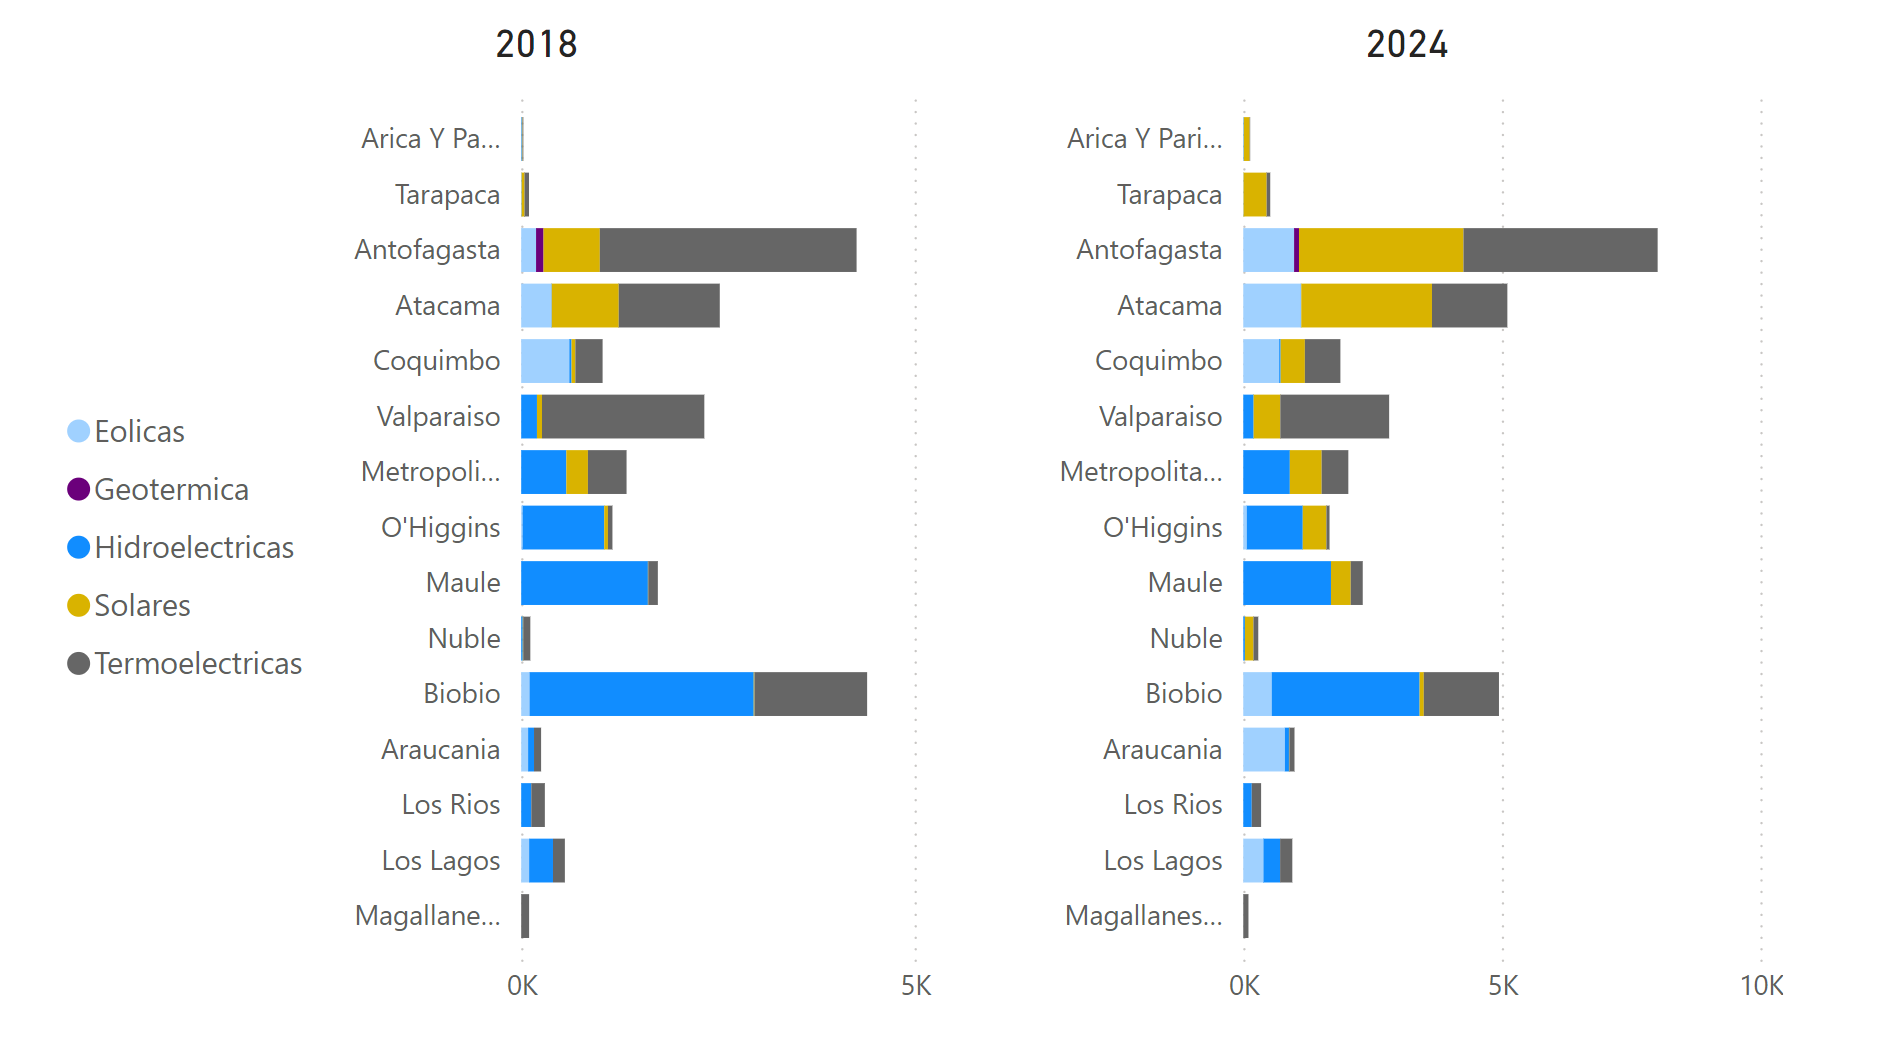
\includegraphics[width=1\columnwidth]{matriz_sist.png}
    \caption{Cambio en la Matriz de Generación del SEN}
    \label{fig:matriz_sistema}
\end{figure}

\paragraph{}
La disminución de la producción y la baja de los CMg afectan por partida doble la rentabilidad de las centrales ERNC, ya que
no solo inyectan menos energía, sino que la que logran entregar al sistema se vende a costo muy bajo o 0.
Estas escenario ha generado otro boom en la industria, que busca aminorar estos efectos a traves del desarrollo de 
proyectos de almacenamiento de energía (BESS) que les permitirá almacenar la energía generada en horas de exceso de esta 
e inyectarla en horas donde hay mejores precios. Pero para rentabilizar estos proyectos es necesario maximizar el spread
del CMg, es decir, comprar la energía en las horas de menor precio y luego venderla en las de mayor CMg. Para esto,
trabajaremos con distintos modelos, de modo de identificar la arquitectura que mejor se adapte a la tarea del pronóstico 
de los costos.

\begin{figure}[htbp]
    \centering
    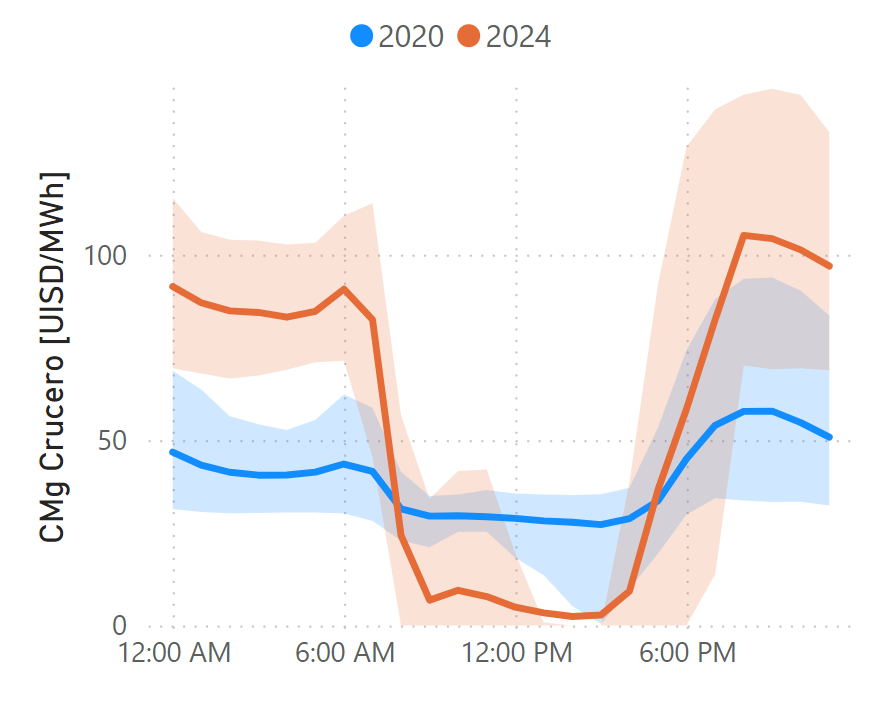
\includegraphics[width=0.8\columnwidth]{cmg_comparacion.png}
    \caption{Comparación perfil diario CMg promedio pre y post escenario de congestión em barra
	Crucero 220kV}
    \label{fig:comp_cmg}
\end{figure}


\section{Metodología}

\subsection{Datos}
Para la el entrenamiento de los modelos, contamos con una serie de datos
los cuales son considerados drivers claves del costo marginal, adicionales al CMg histórico
el cual será nuestra variable objetivo.

\begin{itemize}
    \item Demanda Nacional
    
    Valores historicos de la demanda electrica nacional en MW desde el 2018 a la fecha y con
	resolución horaria.

    \item Disponibilida ERNC
    
    Pronóstico histórico de la disponibilidad de ERNC en MW por central 
	desde el 2018 a la fecha y con
	resolución horaria.

    \item Matriz de Generación
    
	Potencia instalada por tecnología en MW a lo largo del tiempo desde 2018 hasta la fecha.

    \item Cotas de Embalse
    
	Cotas de embalse de las principales centrales hidroeléctricas del sistema.
\end{itemize}

La combinación de estos datos, con distintas escalas de estaicionalidad, nos entregarán unas condiciones
de borde importantes para el pronóstico del CMg.

\subsection{Modelos}
Para abordar el problema, se compararan tres arquitecturas de deep learning, en las que se busca
un enfoque novedoso para enfrentar este problema de series de tiempo:

\begin{enumerate}
    \item GCN + GRU

	Combina una GCN para modelar la red de transmisión, capturando interacciones espaciales, con 	una capa GRU para dependencias temporales.

    \item Informer
    
	Transformer optimizado para series largas, ideal para detectar patrones de largo alcance en la 	demanda y disponibilidad energética.
    \item Transformers + CNN para Series Temporales

	Utiliza CNN para estacionalidades de corto plazo y atención para relaciones de largo plazo, 		adaptándose a la variabilidad del CMg en contextos de alta congestión.
    
\end{enumerate}

\section{Conclusión}
Este proyecto proporciona un enfoque comparativo para la predicción del CMg en el sistema energético chileno, utilizando arquitecturas avanzadas de deep learning. A través del análisis del rendimiento de GCN + GRU, Informer y TFT, esperamos identificar la arquitectura que mejor capte la complejidad espaciotemporal del CMg, optimizando el arbitraje en BESS y aportando un nuevo enfoque para el manejo de la volatilidad en sistemas energéticos.



% \section{Conclusions}\label{conclusions}
% There is no longer \LaTeX{} example which was written by \cite{doe}.


% \begin{thebibliography}{9}
% \bibitem[Doe]{doe} \emph{First and last \LaTeX{} example.},
% John Doe 50 B.C. 
% \end{thebibliography}

\end{document}